\part{Conception d'ensemble}
\setcounter{section}{0}

\section{Modèles conceptuels de données} 

\subsection{Données clients et produits} 

\begin{figure}[H]
\centering
\includegraphics[width=0.8\textwidth]{figures/mcd/MCD_Clients_Produits}
\caption{MCD Clients Produits}
\end{figure}

On a distingué quatre proximités au niveau de la sémantique des données, le client, la personne, le produit et la structure. \\

Tout ce qui est du domaine de l'humain est dans l'objet métier \textbf{Personne}, soit l'individu ainsi que son ou ses lieux d'habitation. À ne pas mélanger avec les différents individus qui ont un rôle, comme l'agent et le client. Le cycle de vie d'une personne est bien différent de celui du rôle qu'elle joue. \\

Ce qui est du domaine des produits et des services sont regroupés dans l'objet métier \textbf{Produit}. On y trouve l'entité produit avec ses offres associées et la segmentation des individus qui est primordiale pour une offre (proximité fonctionnelle). \\

Toute la structuration de la société, soit les agences et les agents y travaillant ont aussi été rapprochés afin de former l'objet métier \textbf{Structure}. Même si le cycle de vie peut différer, on a une proximité fonctionnelle. Ainsi pour limiter les interactions entre blocs nous avons fait le choix de le laisser regroupé ainsi. \\

Enfin, une personne ayant le rôle de client n'existe que si cette dernière possède des comptes, donc la sémantique des données est très proche. On a alors l'objet métier \textbf{Client}. Il est plus pertinent de garder les différentes associations multiples (\textit{0,n}) entre \textbf{Client} et les autres blocs, car c'est lui qui est au centre. On aura par exemple plus de liaison dans le sens \textbf{Client} / \textbf{Produit} que l'inverse.

\subsection{Données commerciales}

\begin{figure}[H]
\centering
\includegraphics[width=0.8\textwidth]{figures/mcd/MCD_Commercial}
\caption{MCD Commercial}
\end{figure}

On retrouve les objets métiers du découpage précédent (\textbf{Client}, \textbf{Produit} et \textbf{Structure}) avec trois autres blocs : \textbf{Agenda}, \textbf{Événement} et \textbf{Contact}. \\

Nous avons dissocié l'entité événement de l'ensemble du domaine des données concernant les contacts, car d'après le cas d'utilisation numéro un, ces derniers sont générés automatiquement en fonction des événements donc ils ont un cycle de vie différent. L'association "Avoir origine" se retrouve avec l'objet métier \textbf{Événement} car on a plus d'accès à partir de l'événement que de l'objet client (du fait du processus de génération automatique). \\

Concernant la planification, nous retrouvons trois entités \textit{Plage agenda}, \textit{Type activité} et \textit{Tâche élémentaire}, c'est pourquoi on retrouve ces entités dans l'objet métier \textbf{Agenda}. Nous avons rajouté l'association \textit{Composer} dans ce bloc car d'après les cas d'utilisations, l'accès aux contacts se fait principalement depuis l'agenda et peu dans l'autre sens. \\

Enfin, nous avons estimé que les entités restantes sont du domaine du \textbf{Contact} et qu'il est plus optimal d'avoir l'ensemble des associations restantes dans cet objet métier car d'après les cas d'utilisation un contact dépend d'un client, un événement, un agent et un ensemble de produit proposés pour ce contact. \\

Afin de simplifier la gestion des entités contacts réalisés et contacts prévus, nous avons fait le choix de nommer cet ensemble \textit{Contact} pour les diagrammes de séquence. On retrouve ainsi pour un contact prévu l'ensemble des contacts réalisés associés. \\

Nous avons fait le choix d'ajouter une association réflexive dans l'entité contact car il faut stocker l'information lorsque plusieurs contacts sont regroupés en un seul. On garde alors l'ensemble des contacts avec les motifs associés et on a cette nouvelle information. \\

Pour terminer, pour des raisons pratiques, il est intéressant d'avoir les informations sur le temps au niveau d'un contact réalisé, c'est pourquoi nous avons ajouté l'association "Effectuer le" pour pouvoir la garder. \\

\section{Diagramme d’état de l'objet métier \bf{contact}}

Le diagramme d'état suivant décrit le cycle de vie complet de l'objet \sc{Contact}. Le cas nominal concernant l'objet métier \sc{Contact} est le suivant, l'objet est créé automatiquement par le système suite à l'apparition d'un évènement entrainant sa création. Après cette action, l'objet contact est dans l'état \bf{PREVU}. Après affectation par le chef d'agence, l'objet \sc{Contact} atteint l'état \bf{AFFECTE} qui fait partie du super état \bf{EN TRAITEMENT}. L'agent est alors chargé de prendre rendez-vous avec le client ce qui a pour effet de faire passer le \sc{Contact} dans l'état \bf{RDV PRIS}. Depuis cet état l'agent peut préparer l'entretien et faire passer l'objet \sc{Contact} dans l'état \bf{PREPARE} puis conduire l'entretien et atteindre l'état \bf{REALISE} ou conduire l'entretien sans l'avoir préparé et atteindre directement \bf{REALISE}. Une fois dans cet état, l'objet \sc{Contact} n'évolue plus. \\
Quelques cas particuliers peuvent intervenir dans la vie de l'objet. Un \sc{Contact} peut être créé directement dans l'état \bf{RDV PRIS} sur contact spontané de la part du client. De même l'agent peut annuler le rendez-vous dans les états \bf{RDV PRIS} et \bf{PREPARE} faire passer l'objet \sc{Contact} dans l'état \bf{AFFECTE}. Enfin, l'agent peut annuler définitivement le contact depuis les états contenus dans le super état \bf{EN TRAITEMENT} ce qui a pour effet de faire passer l'objet \sc{Contact} dans l'état \bf{ANNULE} où il n'évolue plus.

\begin{figure}[H]
\noindent\makebox[\textwidth]{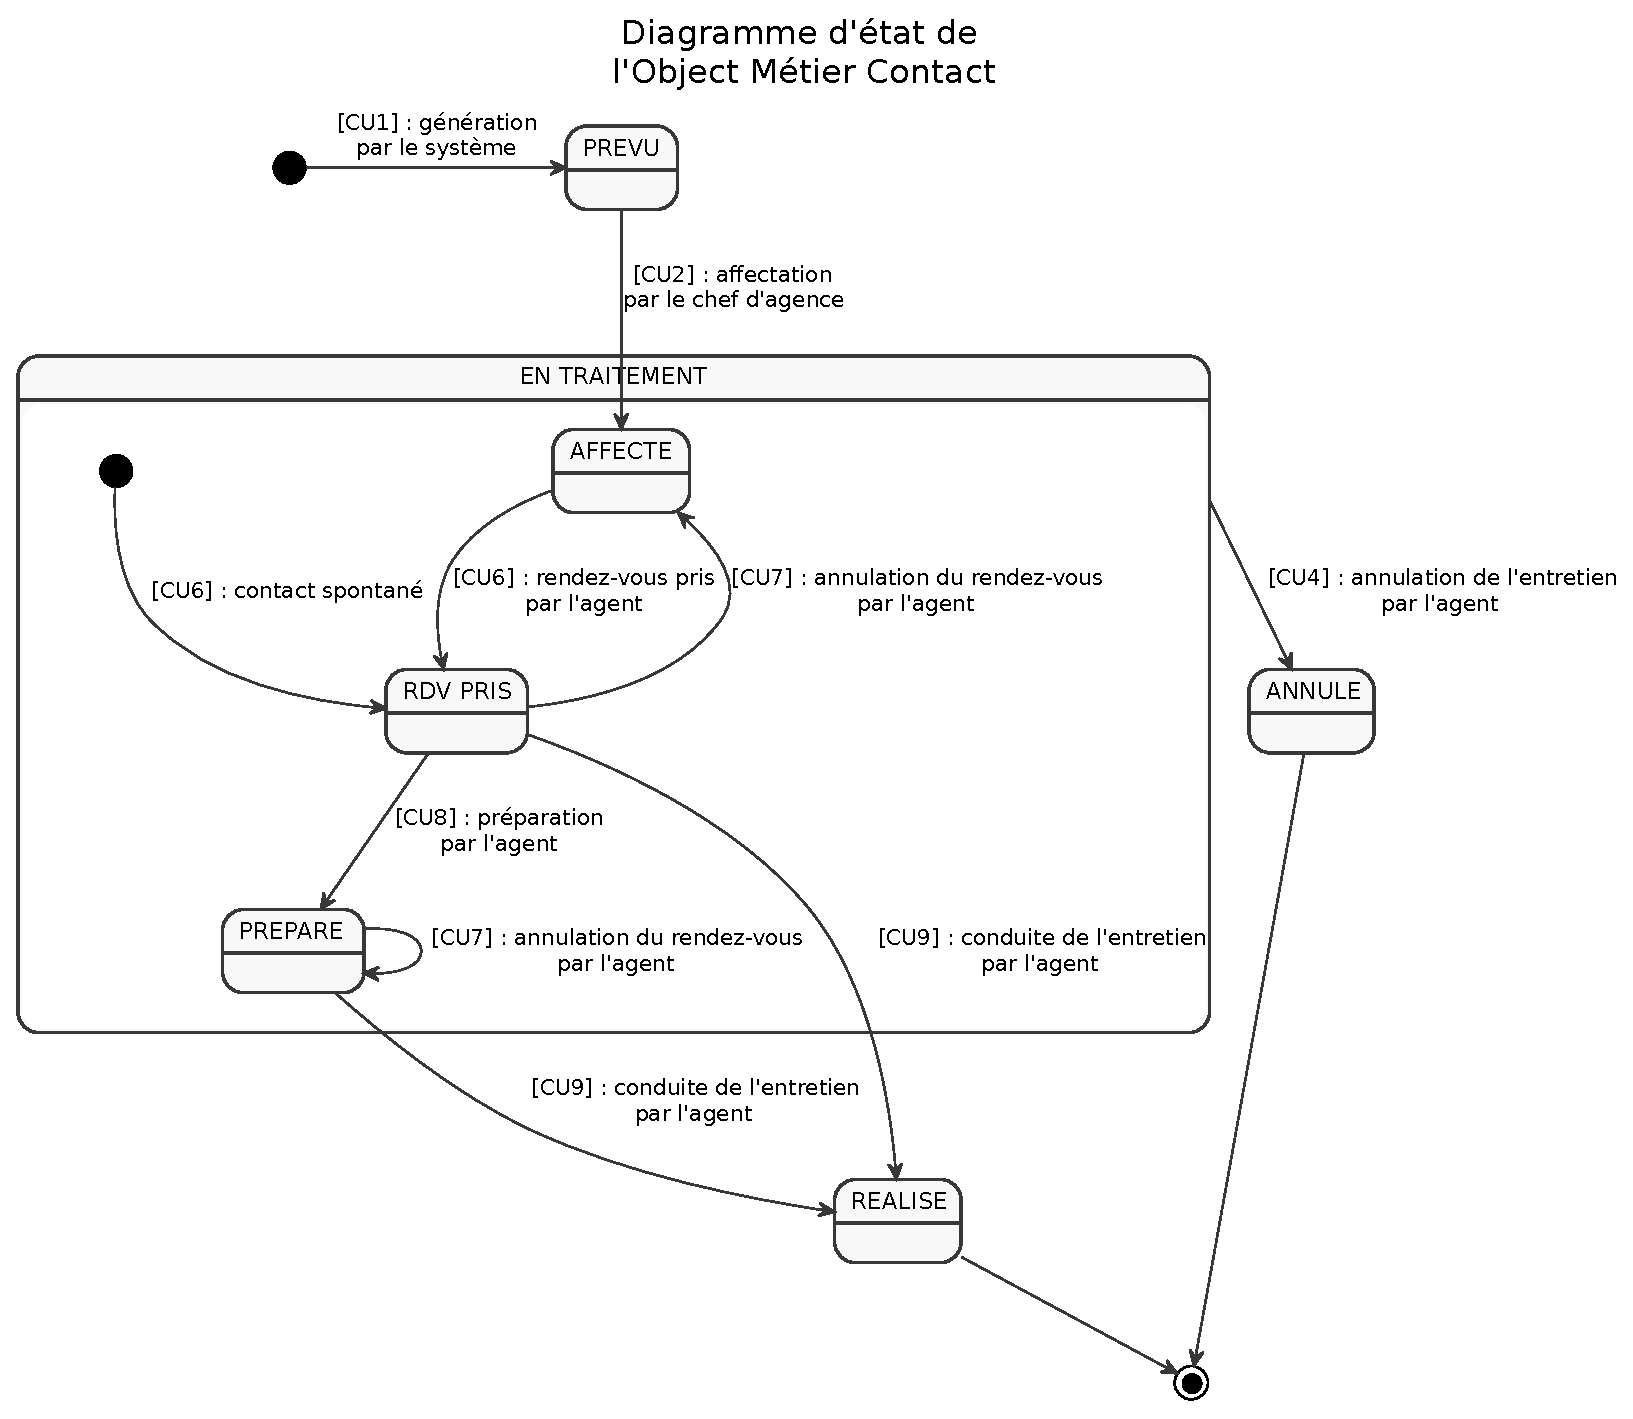
\includegraphics[width=18cm]{figures/eps/diag_etats_contact}}
\caption{Diagramme d'état de l'objet métier contact}
\end{figure}

\section{Choix  de  l’environnement  technique}
L’environnement  technique  déjà  retenu  par  la 
Maîtrise d’Ouvrage (MOA) de la banque est une architecture C/S n-tiers. 
